\let\clearpage\relax

\begin{textbox}{\href{https://compneuro.neuromatch.io/tutorials/W1D4_DimensionalityReduction/student/W1D4_Tutorial1.html}{Dimensionality Reduction } }
\begin{subbox}{subbox}{Generate Correlated Multivariate Data}
\scriptsize
 Multivariate data can be visualized as a cloud of points in a high-dimensional vector space. The geometry of this cloud is shaped by the covariance matrix.

The covariance can be found from the equation above:

\begin{align}
\text{cov}(x_1,x_2) = \rho \sqrt{\sigma_1^2 \sigma_2^2}.
\end{align}
The covariance matrix for two dimensions has the following form:

\begin{align}
{\bf \Sigma} = 
\begin{pmatrix}
 \text{var}(x_1) & \text{cov}(x_1,x_2) \\
 \text{cov}(x_1,x_2) &\text{var}(x_2)
\end{pmatrix}.
\end{align}

\centering
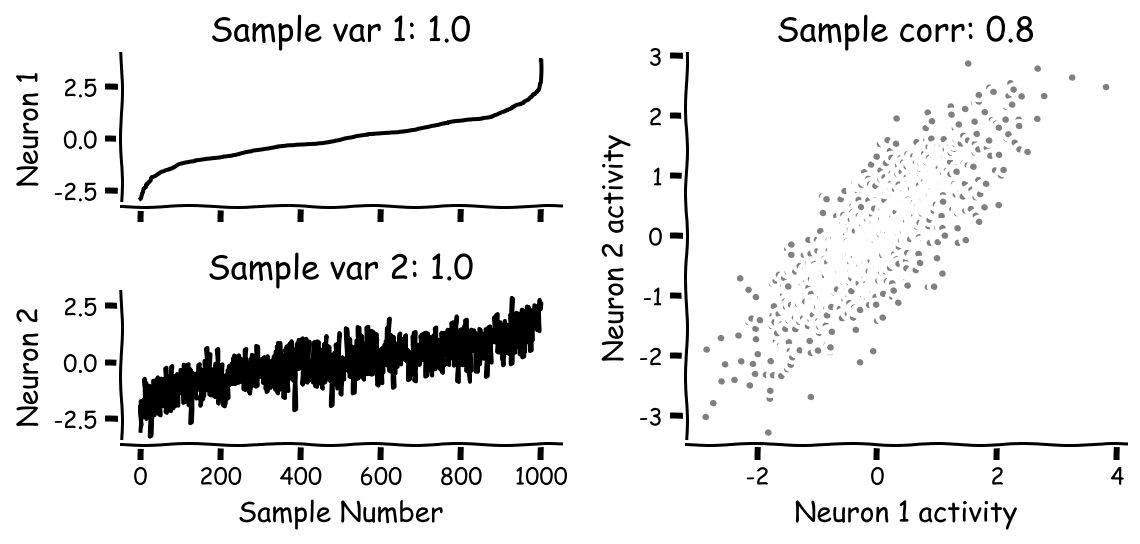
\includegraphics[scale=0.15]{Figures/DM/DMFigure1.png}
\end{subbox}

\begin{subbox}{subbox}{Orthonormal Basis
}
\scriptsize
Two vectors are orthonormal if: 
\begin{enumerate}
    \item 
   They are orthogonal (i.e., their dot product is zero):
\begin{align}
{\bf u\cdot w} = u_1 w_1 + u_2 w_2 = 0
\end{align}
\item   They have unit length:
\begin{align}
||{\bf u} || = ||{\bf w} || = 1
\end{align}
\end{enumerate}
\centering
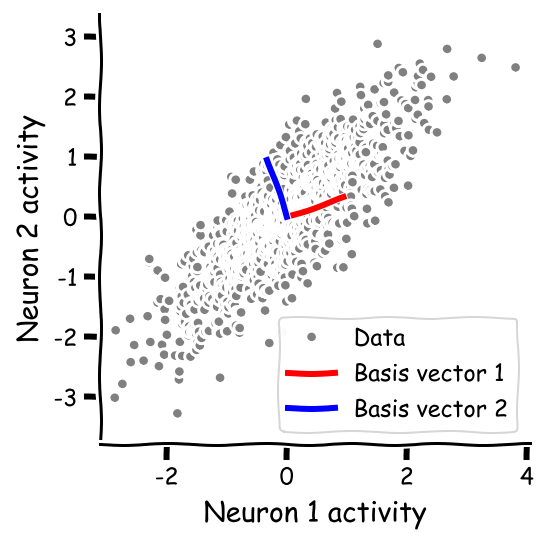
\includegraphics[scale=0.18]{Figures/DM/DMFigure2.png}

\end{subbox}
\end{textbox}
%%%%%%%%%%%%%%%%%%%%%%%%%%%%%%%%%%%%%%%%%%%%%%%%%%%%%%%
%%%%%%%%%%%%%%%%%%%%%%%%%%%%%%%%%%%%%%%%%%%%%%%%%%%%%%%
\begin{textbox}{\href{https://compneuro.neuromatch.io/tutorials/W1D4_DimensionalityReduction/student/W1D4_Tutorial2.html}{Principal Component Analysis } }
\begin{subbox}{subbox}{Eigenvectors of the Sample Covariance Matrix}
\scriptsize
PCA represents data in a new orthonormal basis defined by the eigenvectors of the covariance matrix. The bivariate normal data with a specified covariance matrix $\bf \Sigma$, whose $(i,j)$th element is:
\begin{align}
\Sigma_{ij} = \mathbb{E}[ x_i x_j ] - \mathbb{E}[ x_i] \mathbb{E}[ x_j ] .
\end{align}
 We use the sample covariance matrix, $\bf\hat\Sigma$, which is calculated directly from the data. The $(i,j)$th element of the sample covariance matrix is:
\begin{align}
 \hat \Sigma_{ij} =  \frac{1}{N_\text{samples}}{\bf x}_i^T {\bf x}_j - \bar {\bf x}_i \bar{\bf x}_j ,
\end{align}
where ${\bf x}_i = [ x_i(1), x_i(2), \dots,x_i(N_\text{samples})]^T$ is a column vector representing all measurements of neuron $i$, and  $\bar {\bf x}_i$ is the mean of neuron $i$ across samples:
\begin{align}
\bar {\bf x}_i = \frac{1}{N_\text{samples}} \sum_{k=1}^{N_\text{samples}} x_i(k).
\end{align}
If we assume that the data has already been mean-subtracted, then we can write the sample covariance matrix in a much simpler matrix form:
\begin{align}
{\bf \hat \Sigma}
&= \frac{1}{N_\text{samples}} {\bf X}^T {\bf X}.
\end{align}

where $\bf X$ is the full data matrix (each column of $\bf X$ is a different $\bf x_i$). 
\end{subbox}

\end{textbox}
%%%%%%%%%%%%%%%%%%%%%%%%%%%%%%%%%%%%%%%%%%%%%%%%%%%%%
%%%%%%%%%%%%%%%%%%%%%%%%%%%%%%%%%%%%%%%%%%%%%%%%%%%%%
\begin{textbox}{\href{https://compneuro.neuromatch.io/tutorials/W1D4_DimensionalityReduction/student/W1D4_Tutorial2.html}{Principal Component Analysis } }

\begin{subbox}{subbox}{PCA by projecting data onto the eigenvectors
}
\scriptsize
To perform PCA project the data onto the eigenvectors of the covariance matrix, i.e.:
\begin{align}
\bf S = X W
\end{align}
where $\bf S$ is an $N_\text{samples} \times N$ matrix representing the projected data (also called \textit{scores}), and $\bf W$ is an $N\times N$ orthogonal matrix, each of whose columns represents the eigenvectors of the covariance matrix (also called \textit{weights} or \textit{loadings}). 
Since $\bf W$ is an orthogonal matrix, ${\bf W}^{-1} = {\bf W}^T$. So by multiplying by ${\bf W}^T$ on each side we can rewrite this equation as  
\begin{align}
{\bf X = S W}^T.
\end{align}
To reconstruct the data from a low-dimensional approximation, we just have to truncate these matrices.  Let's denote ${\bf S}_{1:K}$ and ${\bf W}_{1:K}$ the matrices with only the first $K$ columns of $\bf S$ and $\bf W$, respectively. Then our reconstruction is:
\begin{align}
{\bf \hat X = S}_{1:K} ({\bf W}_{1:K})^T.
\end{align}
\end{subbox}
\end{textbox}
%%%%%%%%%%%%%%%%%%%%%%%%%%%%%%%%%%%%%%%%%%%%%%%%%%%%%
%%%%%%%%%%%%%%%%%%%%%%%%%%%%%%%%%%%%%%%%%%%%%%%%%%%%%
\begin{textbox}{\href{https://compneuro.neuromatch.io/tutorials/W1D4_DimensionalityReduction/student/W1D4_Tutorial3.html}{Dimensionality Reduction \& Reconstruction } }
\begin{subbox}{subbox}{Scree Plot}
\scriptsize

Each eigenvalue describes the variance of the data projected onto its corresponding eigenvector. This is an important concept because it allows us to rank the PCA basis vectors based on how much variance each one can capture in a scree plot.
A scree plot is used to help choose which and how many components to use:

\centering
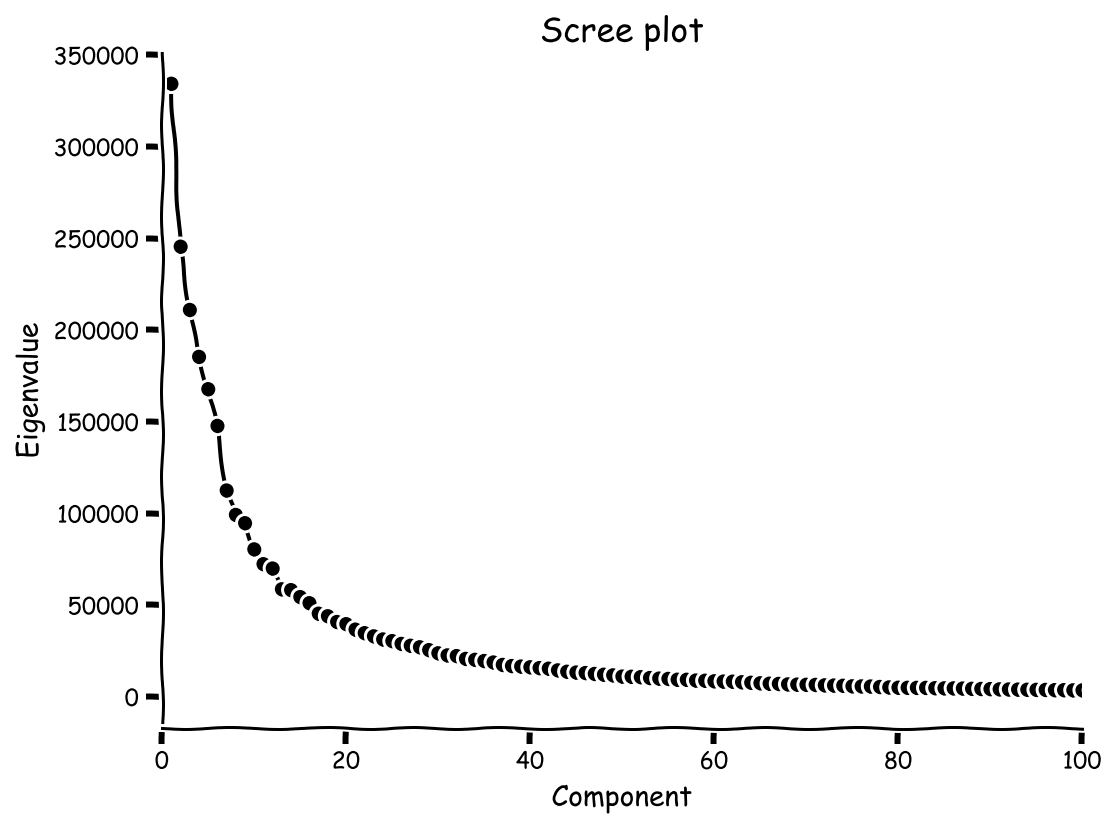
\includegraphics[scale=0.13]{Figures/DM/DMFigure3.png}

\end{subbox}

\begin{subbox}{subbox}{Calculate the variance explained
}
\scriptsize
Another common way to determine the intrinsic dimensionality is by considering the variance explained. This can be examined with a cumulative plot of the fraction of the total variance explained by the top $K$ components, i.e.,
\begin{align}
\text{var explained} = \frac{\sum_{i=1}^K \lambda_i}{\sum_{i=1}^N \lambda_i}
\end{align}
where $\lambda_i$ is the $i^{th}$ eigenvalue and $N$ is the total number of components (the original number of dimensions in the data).
The intrinsic dimensionality is often quantified by the $K$ necessary to explain a large proportion of the total variance of the data (often a defined threshold, e.g., 90\%).

\centering
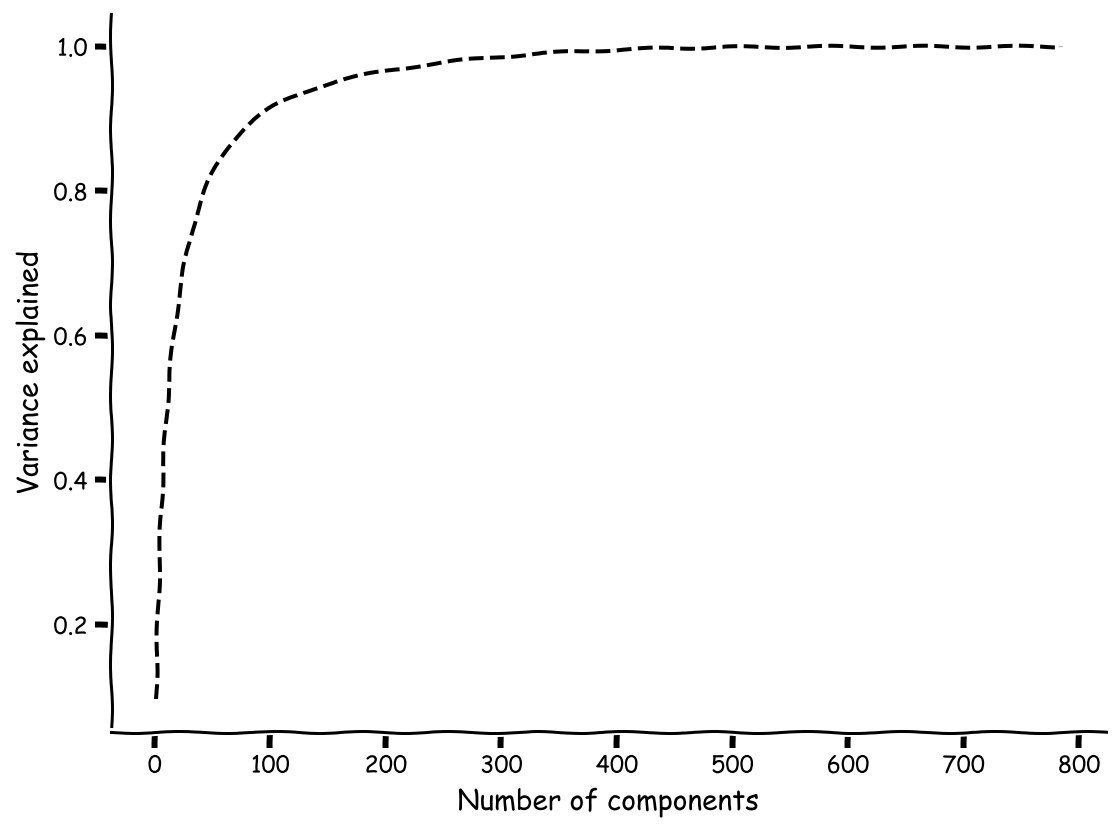
\includegraphics[scale=0.15]{Figures/DM/DMFigure4.png}

\end{subbox}

\end{textbox}
%%%%%%%%%%%%%%%%%%%%%%%%%%%%%%%%%%%%%%%%%%%%%%%%%%%%
%%%%%%%%%%%%%%%%%%%%%%%%%%%%%%%%%%%%%%%%%%%%%%%%%%%%
\begin{textbox}{\href{https://compneuro.neuromatch.io/tutorials/W1D4_DimensionalityReduction/student/W1D4_Tutorial4.html}{ Nonlinear Dimensionality Reduction } }
\begin{subbox}{subbox}{Unsupervised Reduction}
\scriptsize
We will compare PCA with t-SNE, a nonlinear dimensionality reduction method.
Nonlinear methods can be more powerful, they can also be sensitive to noise. In contrast, linear methods are useful for their simplicity and robustness.
Comparing PCA and t-SNE for data visualization. Using t-SNE, we could visualize clusters in the data corresponding to different digits. While PCA was able to separate some clusters (e.g., 0 vs 1), it performed poorly overall.
However, the results of t-SNE can change depending on the choice of perplexity.

\end{subbox}
\begin{subbox}{subbox}{Visualize MNIST in 2D using PCA}
\scriptsize

\centering
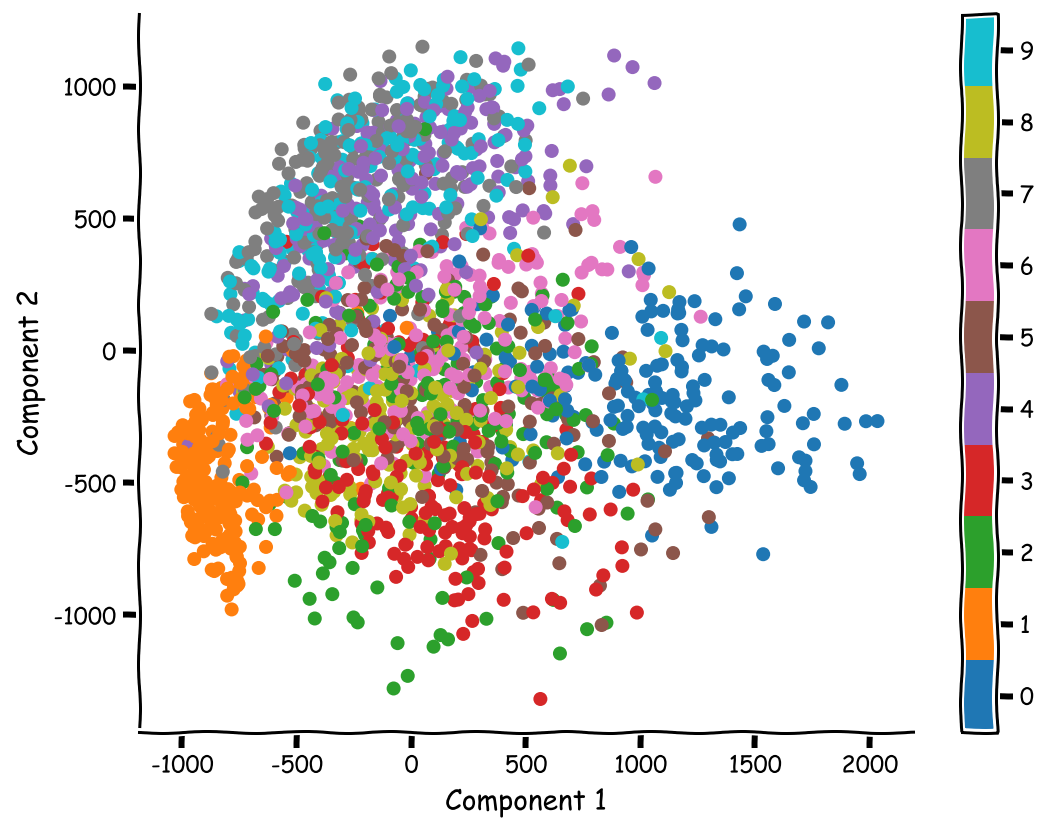
\includegraphics[scale=0.15]{Figures/DM/DMFigure5.png}

\end{subbox}
\begin{subbox}{subbox}{Visualize MNIST in 2D using t-SNE}
\scriptsize

\centering
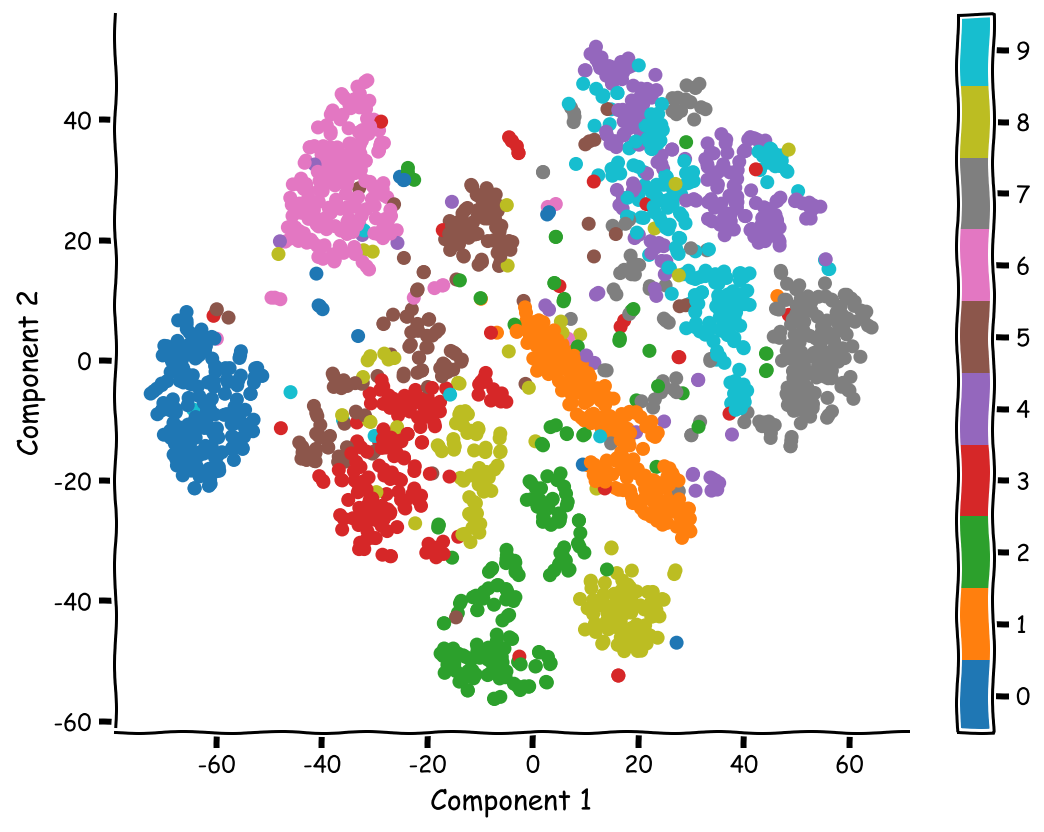
\includegraphics[scale=0.15]{Figures/DM/DMFigure6.png}

\end{subbox}

\end{textbox}